% Harus dimuat terlebih dahulu, digunakan agar file PDF memiliki format karakter yang benar.
% Untuk informasi lebih lanjut, lihat https://ctan.org/pkg/cmap.
\RequirePackage{cmap}

% Format dokumen sebagai paper konferensi menggunakan aturan IEEEtran terbaru (v1.8b).
% Untuk informasi lebih lanjut, lihat http://www.michaelshell.org/tex/ieeetran/.
\documentclass[conference]{IEEEtran}[2015/08/26]

% Format encoding font dan input menjadi 8-bit UTF-8.
\usepackage[T1]{fontenc}
\usepackage[utf8]{inputenc}

% Format bahasa menjadi bahasa german dan inggris.
\usepackage[indonesian]{babel}

% Digunakan untuk tujuan demonstrasi.
\usepackage{mwe}

% Digunakan untuk menampilkan font dengan style yang lebih baik.
\usepackage[zerostyle=b,scaled=.75]{newtxtt}

% Digunakan untuk menampilkan tabel dengan style yang lebih baik.
\usepackage{booktabs}

% Digunakan untuk menampilkan gambar pada dokumen.
\usepackage{graphicx}

% Digunakan untuk menampilkan potongan kode.
\usepackage{listings}
\lstset{
  basicstyle=\ttfamily,
  columns=fixed,
  basewidth=.5em,
  xleftmargin=0.5cm,
  captionpos=b
}

% Digunakan agar backticks (`) dapat dirender pada PDF.
% Untuk informasi lebih lanjut, lihat https://tex.stackexchange.com/a/341057/9075.
\usepackage{upquote}

% Digunakan untuk menyeimbangkan bagian akhir dokumen dengan dua kolom.
\usepackage{balance}

% Digunakan untuk menampilkan pustaka.
\usepackage[square,comma,numbers,sort&compress]{natbib}

% Mengubah format ukuran teks pada natbib.
\renewcommand{\bibfont}{\normalfont\footnotesize}

% Menambah nama penulis ketika menggunakan perintah \citet.
% Untuk informasi lebih lanjut, lihat https://tex.stackexchange.com/a/76075/9075.
\usepackage{etoolbox}
\makeatletter
\patchcmd{\NAT@test}{\else \NAT@nm}{\else \NAT@hyper@{\NAT@nm}}{}{}
\makeatother

% Digunakan untuk melakukan linewrap pada pustaka dengan url yang panjang
% jika terdapat hyphens
\usepackage[hyphens]{url}

% Digunakan untuk menambah hyperlink pada referensi.
\usepackage{hyperref}

% Menonaktifkan warna dan bookmark pada hyperref.
\hypersetup{hidelinks,
  colorlinks=true,
  allcolors=black,
  pdfstartview=Fit,
  breaklinks=true
}

% Digunakan untuk membenarkan hyperref pada gambar.
\usepackage[all]{hypcap}

% Digunakan untuk menampilkan beberapa gambar
\usepackage[caption=false,font=footnotesize]{subfig}

\usepackage{stfloats}

% Tambahkan format tanda hubung yang benar di sini
\hyphenation{
  ro-ket
  me-ngem-bang-kan
  per-hi-tu-ngan
}

\begin{document}

  % Ubah kalimat berikut sesuai dengan judul penelitian.
\title{Kalkulasi Energi pada Roket Luar Angkasa \\ Berbasis \emph{Anti-Gravitasi}}

% Ubah kalimat-kalimat berikut sesuai dengan nama, institusi, alamat dan kontak penulis.
\author{
  \IEEEauthorblockN{Elon Reeve Musk}
  \IEEEauthorblockA{Departemen Teknik Dirgantara\\
    Fakultas Teknologi Dirgantara\\
    Institut Teknologi Sepuluh Nopember\\
    Surabaya, Indonesia 60111\\
    elon.musk@mhs.its.ac.id}

  \and
  \IEEEauthorblockN{Nikola Tesla}
  \IEEEauthorblockA{Departemen Teknik Dirgantara\\
    Fakultas Teknologi Dirgantara\\
    Institut Teknologi Sepuluh Nopember\\
    Surabaya, Indonesia 60111\\
    \url{https://nikolatesla.me}}

  \and
  \IEEEauthorblockN{Wernher von Braun}
  \IEEEauthorblockA{Departemen Teknik Dirgantara\\
    Fakultas Teknologi Dirgantara\\
    Institut Teknologi Sepuluh Nopember\\
    Surabaya, Indonesia 60111\\
    von.braun@td.its.ac.id}
}

% Digunakan untuk menampilkan judul dan deskripsi penulis.
\maketitle

  % Mengubah keterangan `Abstract` ke bahasa indonesia.
% Hapus bagian ini untuk mengembalikan ke format awal.
\renewcommand\abstractname{Abstrak}

\begin{abstract}

  % Ubah paragraf berikut sesuai dengan abstrak dari penelitian.
  \emph{Face detection algorithms nowadays have developed rapidly. 
  This is inseparable from the need for face detection algorithms as an authentication tool and biometric-based security system. 
  However, the main problem of the face detection algorithm is the accuracy that could vary according to environmental conditions. 
  In this final project, we analyze performance of face detection algorithm based on pyramid feature 
  in the surveillance environment. 
  The analysis was carried out with CCTV video as input for the face detection 
  algorithm and carried out with several different scenarios. 
  Some of the scenarios carried out are light conditions, 
  movement of people, multiple face detection, and face detection in disguise. 
  In this research, the latest face detection method based on feature pyramid is used. 
  The main metric used to evaluate the face detection algorithm method based on feature pyramid is 
  mean average precision (mAP) by comparing manual labeling conditions and labeling conditions obtained 
  from the face detection system. 
  In terms of processing time, 
  frame rate per second (FPS) will be used for evaluation under different hardware configuration conditions. 
  The results show that the mobilenet0.25 backbone in the feature pyramid-based face detection system excels in processing time 
  and FPS parameters in all scenarios that are run, while the resnet50 backbone excels in accuracy parameters (mAP) in scenarios where the mobilenet0.25 backbone is difficult to perform detection.}

\end{abstract}

% Mengubah keterangan `Index terms` ke bahasa indonesia.
% Hapus bagian ini untuk mengembalikan ke format awal.
% \renewcommand\IEEEkeywordsname{Kata kunci}

\begin{IEEEkeywords}

  % Ubah kata-kata berikut sesuai dengan kata kunci dari penelitian.
  System Performance Evaluation, Face Detection System, Feature Pyramid Network

\end{IEEEkeywords}


  % Ubah bagian berikut sesuai dengan konten-konten yang akan dimasukkan pada dokumen
  % Ubah judul dan label berikut sesuai dengan yang diinginkan.
\section{Introduction}
\label{sec:pendahuluan}

% Ubah paragraf-paragraf pada bagian ini sesuai dengan yang diinginkan.

Face detection algorithm with high accuracy and fast performance is needed
at this time. This is inseparable from the need for face detection algorithms to
implemented as an identity authentication tool and a biometric-based security system.
Biometrics is an automatic identification system of individuals based on physical and/or physical characteristics
behavioral characteristics in individuals such as fingerprints, faces, irises, or voice \citep{doi:10.1080/09505431.2018.1519534}.
Biometrics were chosen because they have a unique feature, namely they cannot be transferred (non-transferable characteristic) because biometrics
recording physical conditions and/or behavioral conditions in individuals, it is more
reliable compared to legacy authentication systems such as passwords or PINs that only record numbers
or certain letters \citep{1597098}. Therefore, at this time many biometric systems have been developed
on the security system to switch from authentication systems such as passwords and PINs. Compared to the type of biometric that does the recording
Based on physical characteristics, Biometrics using the face is currently still an area
research since 1960 with a wide scope for continuous improvement \citep{zufar}.

More and more methods are being created, making face detection systems more sophisticated today.
There are several methods that can be used according to the required conditions. But basically
real-time conditions with fast computing processes are the main goals of developments
the method. The Deep Learning method that is widely used and developed in face detection algorithms is
CNN based method. CNN is a method inspired by Neural Network (NN) which can solve
a problem with passing an input X into the Convolutional filter circuit and other nonlinear computations \citep{lecun1989handwritten}.
The development of the most recent CNN-based face detection method is one of the facial detection methods based on the feature pyramid. Fundamental difference
of the feature pyramid based face detection method when compared to other face detection methods is the feature pyramid-based face detection method
perform the process of obtaining a feature map with a high semantic level using the feature pyramid network architecture \citep{lin2017feature}. 
The advantage of the feature pyramid-based face detection method is that it can accurately detect the face area of each individual 
in the condition of many faces in one image or frame.

With many methods that have been developed, the face detection algorithm still has challenges from aspects of the detection process
These aspects are the condition of facial variations that vary between individuals, and the size of the face that depends on the distance and search space \citep{Li_2015_CVPR}.
Based on this, in this final project, an evaluation of the performance of the face detection system using the feature pyramid-based face detection method will be carried out. System
face detection based on feature pyramid will be tested using several scenarios of facial variations in different individuals and environments,
So that the output of this final project obtained the best conditions for detecting.

  % Ubah judul dan label berikut sesuai dengan yang diinginkan.
\section{Penelitian Terkait}
\label{sec:penelitianterkait}

% Ubah paragraf-paragraf pada bagian ini sesuai dengan yang diinginkan.

Beberapa penelitian lain pernah dilakukan seperti yang dirumuskan oleh \citet{newton1687} bahwa \lipsum[5]
Hasil tersebut kemudian menjadi persamaan \ref{eq:hukumpertama}.

% Contoh pembuatan persamaan ilmiah.
\begin{equation}
  \label{eq:hukumpertama}
  \sum \mathbf{F} = 0\; \Leftrightarrow\; \frac{\mathrm{d} \mathbf{v} }{\mathrm{d}t} = 0.
\end{equation}

\lipsum[6-7]

  % Ubah judul dan label berikut sesuai dengan yang diinginkan.
\section{Arsitektur}
\label{sec:arsitektur}

% Ubah paragraf-paragraf pada bagian ini sesuai dengan yang diinginkan.

\subsection{Cetak Biru Roket}
\label{subsec:cetakbiruroket}

Pada cetak biru yang tertera pada Gambar \ref{fig:cetakbiru}. \lipsum[8]

% Contoh input gambar pada kolom.
\begin{figure} [ht]
  \centering
  % Ubah sesuai dengan nama file gambar dan ukuran yang akan digunakan.
  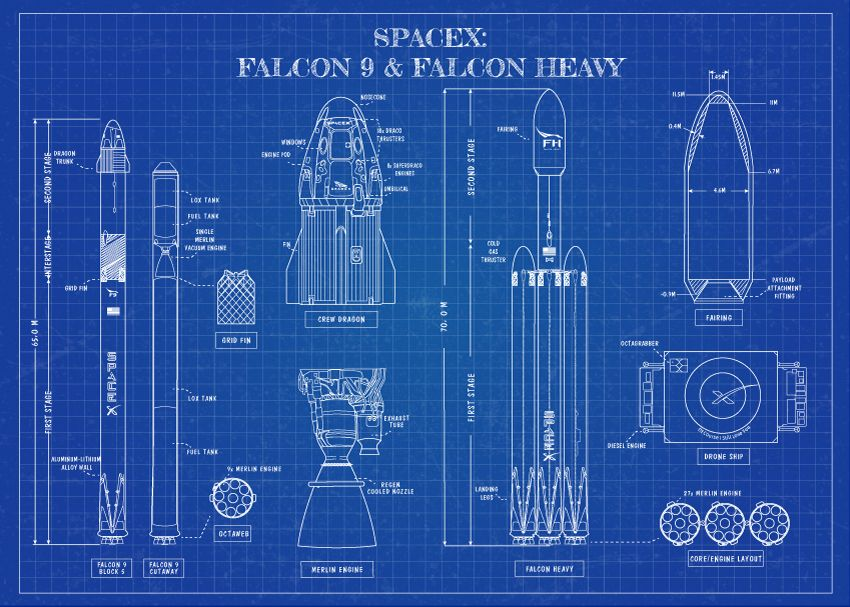
\includegraphics[width=0.4\textwidth]{gambar/cetakbiru.jpg}

  % Ubah sesuai dengan keterangan gambar yang diinginkan.
  \caption{Cetak biru roket yang akan diuji coba. \cite{cetakbiruspacex}}
  \label{fig:cetakbiru}
\end{figure}

\lipsum[9-10]

\subsection{Lorem Ipsum}
\label{subsec:loremipsum}

\lipsum[11]

% Contoh pembuatan tabel.
\begin{table}
  \caption{Contoh tabel sederhana}
  \label{tab:tabelsederhana}
  \centering
  \begin{tabular}{lll}
    \toprule
    Heading1 & Heading2 & Heading3  \\
    \midrule
    One      & Two      & Three     \\
    Four     & Five     & Six       \\
    \bottomrule
  \end{tabular}
\end{table}

% Contoh pembuatan potongan kode.
\begin{lstlisting}[
  language=C++,
  caption={Program halo dunia.},
  label={lst:halodunia}
]
#include <iostream>

int main() {
    std::cout << "Halo Dunia!";
    return 0;
}
\end{lstlisting}

\lipsum[12]

% Contoh pembuatan daftar.
\begin{enumerate}
  \item \lipsum[13][1-4]
  \item \lipsum[13][5-8]
  \item \lipsum[13][9-12]
\end{enumerate}

\lipsum[14-15]

  % % Ubah judul dan label berikut sesuai dengan yang diinginkan.
\section{Testing Parameters}
\label{sec:parameterpengujian}

The evaluation stage is carried out based on the results of face detection by the system.
A face detection system based on feature pyramid network
will provide detection results in the form of confidence and predicted bounding box.
The results of the face detection are then compared with the ground-truth bounding box
previously assigned to the labeling process.
This comparison is done by calculating the value of Intersection over Union (IoU)
or the value of the overlap between ground-truth bounding box
and predicted bounding box.
If the value of IoU of both bounding box
the value is more than the specified threshold,
i.e. 0.5, then the detection result
considered correct. On the other hand, if it turns out that the IoU value obtained
get less than 0.5, then the detection result is considered
wrong.

From the calculation results IoU obtained the value True Positive,
False Positive, and False Negative are used to search for precision and recall values from face detection results.
The Average Precision (AP) value is obtained from the results of calculating the area under the curve of
each class detected by the system. As for the mean value
Average Precision (mAP) is obtained by averaging the AP values of all detected classes.
However, due to
In this research, there is only one class that will be detected, namely face,
it can be concluded that the mAP value
generated is equal to the value of AP.


\subsection{Confusion Matrix}

The Confusion Matrix is one method that can
used to measure the performance of a classification system. 
The confusion matrix contains detailed information regarding the classification (prediction) results by the system on testing data whose class is known
(actual) and are usually arranged in the form of a matrix \citep{haykin2009neural}.

Some of the conditions contained in the confussion matrix for the two classes include:

\begin{enumerate}
  \item True Positive (TP), which is the number of positive data that
  correctly classified by the system.
  \item False Positive (FP), which is the number of negative data that
  classified as positive by the system (type I error).
  \item False Negative (FN), which is the number of positive data that
  classified as negative by the system (type II error).
\end{enumerate}

These conditions are used to perform calculations on other instruments to measure performance
face detection system based on feature pyramid network. These instruments include:

\begin{itemize}
  \item \emph{Precision}
  
  \begin{equation}
    \frac{TP}{TP+FP} 
  \end{equation}
  
  \item \emph{Recall}
  
  \begin{equation}
    \frac{TP}{TP+FN}
  \end{equation}  

  \item \emph{Accuracy}
  
  \begin{equation}
    \frac{TP+TN}{TP+TN+FP+FN}
  \end{equation}  

\end{itemize}

\bigskip

\subsection{Intersection over Union}

Intersection over Union (IoU) is an evaluation metric used to measure
object detection accuracy on a particular dataset \citep{aghdam2017guide}. IoU can be used to assess detection systems
object with the following conditions:

\begin{itemize}
  \item Model generates predictions of (x, y) coordinates, such as bounding box for objects in the image.
  \item Has a ground-truth bounding box in the object's dataset.
  \item Has a predicted bounding box of the model.
\end{itemize}

In general, IoU is used to evaluate HOG+Linear SVM
and CNN-based object detection. However as long as the model has two bounding box sets
in accordance with the provisions of points 2 and
3 above, then IoU can be applied in the model.

IoU is the ratio of the cut area to
the combined area of predicted bounding box and ground-truth bounding box.
Normally, a model can be said to be good if the score
The IoU obtained from the prediction is more than 0.5.

\subsection{mean Average Precision (mAP)}

mean Average Precision (mAP) is an evaluation metric that
measure the accuracy of an object detector in the detection process.
The mAP value is the average of
the value of Average Precision (AP) of each object class. AP got
by calculating the area under the precision-recall curve that
made based on precision and recall values. mAP formula describes as follows:

\begin{equation}
  AP = \sum_n (R_n - R_{n-1}) P_n
  \label{map}
\end{equation}

Where $Pn$ and $Rn$ are the precision and recall at the math th threshold. AP can also be regarded as the area under the precision-recall curve. MAP is the mean of AP over all the queries.
% \begin{equation}
%     % Label referensi dari persamaan yang dibuat
%     \label{eq:IOU}
%     % Baris kode persamaan yang dibuat
%     IOU = (Area of Overlap) / (Area of Union)
% \end{equation}

% Apabila nilai IoU dari kedua bounding box tersebut bernilai
% lebih dari threshold yang ditentukan dalam penelitian ini, yaitu
% 0.5, maka hasil pendeteksian tersebut dianggap benar.
% Sebaliknya, apabila ternyata nilai IoU yang didapatkan kurang
% dari 0.5, maka hasil pendeteksian tersebut dianggap salah. Dari
% hasil penghitungan IoU didapatkan beberapa nilai antara lain:
% \begin{enumerate}
%     \item True Positive (TP), yaitu jumlah data positif yang
%     terklasifikasi benar oleh sistem.
%     \item False Positive (FP), yaitu jumlah data negatif yang
%     terklasifikasi positif oleh sistem (type I error).
%     \item False Negative (FN), yaitu jumlah data positif yang
%     terklasifikasi negatif oleh sistem (type II error).
% \end{enumerate}
% Ketiga nilai tersebut digunakan untuk mencari nilai
% precision dan recall dari hasil pendeteksian wajah. Nilai
% precision dan recall sendiri didapatkan dengan menggunakan
% persamaan:

% Recall dapat dihitung menggunakan rumus:
% \begin{equation}
%   % Label referensi dari persamaan yang dibuat
%   \label{eq:Recall}
%   % Baris kode persamaan yang dibuat
%   \frac{TP}{TP+FN}
% \end{equation}

% Sedangkan Precision dapat dihitung menggunakan rumus:
% \begin{equation}
%   % Label referensi dari persamaan yang dibuat
%   \label{eq:Precision}
%   % Baris kode persamaan yang dibuat
%   \frac{TP}{TP+FP}
% \end{equation}

% Nilai mean Average Precision (mAP) didapatkan dengan
% cara merata-ratakan nilai AP dari seluruh kelas yang terdeteksi.
% Namun, karena pada penelitian ini hanya terdapat satu kelas 
% yang akan dideteksi, yaitu wajah, maka dapat ditarik
% kesimpulan bahwa nilai mAP yang dihasilkan sama dengan
% nilai dari AP

% \begin{equation}
%     % Label referensi dari persamaan yang dibuat
%     \label{eq:MAP}
%     % Baris kode persamaan yang dibuat
%     AP = \sum_n (R_n - R_{n-1}) P_n
% \end{equation}

% % Ubah paragraf-paragraf pada bagian ini sesuai dengan yang diinginkan.

% % Contoh input beberapa gambar pada halaman.
% \begin{figure*}
%   \centering
%   \subfloat[Hasil A]{\includegraphics[width=.4\textwidth]{example-image-a}
%     \label{fig:hasila}}
%   \hfil
%   \subfloat[Hasil B]{\includegraphics[width=.4\textwidth]{example-image-b}
%     \label{fig:hasilb}}
%   \caption{Contoh input beberapa gambar.}
%   \label{fig:hasil}
% \end{figure*}

% \lipsum[16-18]

% % Contoh input potongan kode dari file.
% \lstinputlisting[
%   language=Python,
%   caption={Program perhitungan bilangan prima.},
%   label={lst:bilanganprima}
% ]{program/bilangan-prima.py}

% \lipsum[19-20]

\section{RESULTS AND ANALYSIS}
\label{sec:hasilpembahasan}

In this study, the results of testing several scenarios that have been obtained and analyzing the results are presented.

\subsection{Testing Based on Data Collection Time}

Testing based on the time of data collection aims to find out
effect of data retrieval time and light on computing performance
and face detection results. On testing
This data obtained was taken during the day and night so that the data obtained
under very different light conditions. In this test, there are 24 different scenarios that were carried out previously mentioned.

\begin{table}[pt]
  \caption{Table of detection results based on time (Daylight)}
  \centering
  \resizebox{\columnwidth}{!}{\begin{tabular}{|l|l|l|l|l|l|l|} 
    \hline
    \multicolumn{1}{|c|}{\multirow{2}{*}{\begin{tabular}[c]{@{}c@{}}\textbf{VALUE}\end{tabular}}} & \multicolumn{3}{c|}{\textbf{Backbone Mobilenet0.25 }}                                                                                                                   & \multicolumn{3}{c|}{\textbf{Backbone Resnet50 }}                                                                                                                                           \\ 
    \cline{2-7}
    \multicolumn{1}{|c|}{}                                                                                               & \multicolumn{1}{c|}{\begin{tabular}[c]{@{}c@{}}\textbf{Processing}\\\textbf{Time}\end{tabular}} & \multicolumn{1}{c|}{\textbf{FPS}} & \multicolumn{1}{c|}{\textbf{mAP}} & \multicolumn{1}{c|}{\begin{tabular}[c]{@{}c@{}}\textbf{\textbf{Processing}}\\\textbf{\textbf{Time}}\end{tabular}} & \multicolumn{1}{c|}{\textbf{FPS}} & \multicolumn{1}{c|}{\textbf{mAP}}  \\ 
    \hline
    \textbf{MAX}                                                                                                    & 15.460                                                                                          & 142.534                           & 99.94\%                           & 31.194                                                                                                            & 18.530                            & 100.00\%                           \\ 
    \hline
    \textbf{MIN}                                                                                                     & 11.563                                                                                          & 138.164                           & 25.40\%                           & 21.490                                                                                                            & 18.500                            & 50.79\%                            \\ 
    \hline
    \textbf{AVERAGE}                                                                                                   & 12.615                                                                                          & 138.972                           & 83.32\%                           & 23.488                                                                                                            & 18.514                            & 86.84\%                            \\ 
    \hline
    \textbf{TOTAL}                                                                                                       & 302.749                                                                                         & -                                 & -                                 & 563.709                                                                                                           & -                                 & -                                  \\
    \hline
    \end{tabular}}
  \label{table:pendeteksianberdasarkanwaktusiang}
\end{table}

\begin{table}[pt]
  \caption{Table of detection results based on time (Night)}
  \centering
  \resizebox{\columnwidth}{!}{\begin{tabular}{|l|c|c|c|c|c|c|} 
    \hline
    \multicolumn{1}{|c|}{\multirow{2}{*}{\begin{tabular}[c]{@{}c@{}}\textbf{VALUE}\end{tabular}}} & \multicolumn{3}{c|}{\textbf{Backbone Mobilenet0.25 }}                                                    & \multicolumn{3}{c|}{\textbf{Backbone Resnet50 }}                                                                            \\ 
    \cline{2-7}
    \multicolumn{1}{|c|}{}                                                                                               & \begin{tabular}[c]{@{}c@{}}\textbf{Processing}\\\textbf{Time}\end{tabular} & \textbf{FPS} & \textbf{mAP} & \begin{tabular}[c]{@{}c@{}}\textbf{\textbf{Processing}}\\\textbf{\textbf{Time}}\end{tabular} & \textbf{FPS} & \textbf{mAP}  \\ 
    \hline
    \textbf{MAX}                                                                                                    & 12.724                                                                     & 138.928      & 99.92\%      & 27.389                                                                                       & 18.527       & 100.00\%      \\ 
    \hline
    \textbf{MIN}                                                                                                     & 11.283                                                                     & 137.489      & 70.15\%      & 20.897                                                                                       & 18.497       & 66.44\%       \\ 
    \hline
    \textbf{AVERAGE}                                                                                                   & 12.035                                                                     & 138.265      & 89.74\%      & 23.232                                                                                       & 18.511       & 89.43\%       \\ 
    \hline
    \textbf{TOTAL}                                                                                                       & 288.845                                                                    & -            & -            & 557.562                                                                                      & -            & -             \\
    \hline
    \end{tabular}}
  \label{table:pendeteksianberdasarkanwaktumalam}
\end{table}

This scenario aims to be able to assess which backbone face detection model is based on which feature pyramid
which is superior for easy to difficult face detection in different light conditions.
In the results Table (\ref{table:pendeteksianberdasarkanwaktusiang} and Table \ref{table:pendeteksianberdasarkanwaktumalam}) of backbone mobilenet0.25 are far superior to the FPS parameter
compared to backbone resnet50. The average FPS for backbone mobilenet0.25 was at $138$ FPS, while for backbone resnet50 it was at $18.5$ FPS. But for accuracy, with parameter 
mean average precision (mAP) backbone resnet50 is slightly superior to backbone mobilenet0.25. Backbone resnet50 get the maximum value of mAP at $100\%$ with obstacle condition
only glasses during the day and a hitch of sunglasses, hats, hoodies in night conditions. Another advantage of backbone mobilenet0.25 can be seen from the parameters
Average mAP, The average mAP obtained from backbone mobilenet0.25 is superior to backbone resnet50 in both daytime and daytime conditions.

\subsection{Testing Based on the Number of Objects}

In testing based on the number of objects aimed at
determine the effect of the number of objects on the ability of the system
in detecting faces. The data obtained previously in the form of cctv camera data taken
during the day. There are ten combination conditions mentioned earlier.

\begin{table}[pt]
  \caption{Table of detection results based on number of objects}
  \centering
  \resizebox{\columnwidth}{!}{\begin{tabular}{|l|c|c|c|c|c|c|} 
    \hline
    \multicolumn{1}{|c|}{\multirow{2}{*}{\textbf{VALUE}}} & \multicolumn{3}{c|}{\textbf{Backbone Mobilenet0.25 }}                                                    & \multicolumn{3}{c|}{\textbf{Backbone Resnet50 }}                                                                            \\ 
    \cline{2-7}
    \multicolumn{1}{|c|}{}                                & \begin{tabular}[c]{@{}c@{}}\textbf{Processing}\\\textbf{Time}\end{tabular} & \textbf{FPS} & \textbf{mAP} & \begin{tabular}[c]{@{}c@{}}\textbf{\textbf{Processing}}\\\textbf{\textbf{Time}}\end{tabular} & \textbf{FPS} & \textbf{mAP}  \\ 
    \hline
    \textbf{MAX}                                          & 14.111                                                                     & 139.251      & 92.56\%      & 34.063                                                                                       & 18.598       & 97.49\%       \\ 
    \hline
    \textbf{MIN}                                          & 12.983                                                                     & 137.867      & 79.37\%      & 22.261                                                                                       & 18.504       & 90.38\%       \\ 
    \hline
    \textbf{AVERAGE}                                      & 13.584                                                                     & 138.652      & 88.52\%      & 27.819                                                                                       & 18.534       & 94.70\%       \\ 
    \hline
    \textbf{TOTAL}                                        & 135.844                                                                    & -            & -            & 278.192                                                                                      & -            & -             \\
    \hline
    \end{tabular}}
  \label{table:pendeteksianberdasarkanjumlahobject}
\end{table}

In the results (Table \ref{table:pendeteksianberdasarkanjumlahobject}) of backbone mobilenet0.25 are far superior to backbone resnet50
with FPS parameters. Backbone mobilenet0.25 got an average FPS of $138$ FPS while backbone resnet50 got an average FPS of $18.5$ FPS. However 
backbone resnet50 excels in the average mAP obtained, Backbone resnet50 gets an average mAP of $94.7\%$ while backbone mobilenet0.25 gets an average
mAP is $88.52\%$. This shows that backbone resnet50 is more accurate than backbone mobilenet0.25 despite poorer processing time and FPS.

\subsection{Testing Based on Object Velocity}

In testing based on the speed of a moving object aiming at
to determine the effect of the speed of an object when moving at a certain speed on
the system's ability to detect faces. On testing
This is the data taken during the day.
The speed measure is obtained by measuring the travel time
object from the top to the bottom of the frame, travel time
it is then calculated by the long range of the camera
so that the velocity of the object is obtained \citep{nugrohoevalution2016}. There are three conditions
the speed of moving objects, each of which is tested as much as three
previously mentioned times.

\begin{table}[pt]
  \caption{Table of detection results based on object velocity}
  \centering
  \resizebox{\columnwidth}{!}{\begin{tabular}{|l|c|c|c|c|c|c|c|} 
    \hline
    \multicolumn{1}{|c|}{\multirow{2}{*}{\textbf{SCENARIO}}} & \multicolumn{3}{c|}{\textbf{Backbone Mobilenet0.25}}                                                                                                                                                                                                           & \multicolumn{4}{c|}{\textbf{Backbone Resnet50}}                                                                                                                                                                                                                                                                  \\ 
    \cline{2-8}
    \multicolumn{1}{|c|}{}                                   & \begin{tabular}[c]{@{}c@{}}\textbf{Avg.}\\\textbf{Velocity}\\\textbf{(m/s)}\end{tabular} & \begin{tabular}[c]{@{}c@{}}\textbf{Avg.}\\\textbf{Processing}\\\textbf{Time (s)}\end{tabular} & \begin{tabular}[c]{@{}c@{}}\textbf{Avg.}\\\textbf{FPS}\end{tabular} & \begin{tabular}[c]{@{}c@{}}\textbf{Avg.}\\\textbf{mAP}\end{tabular} & \begin{tabular}[c]{@{}c@{}}\textbf{Avg.}\\\textbf{Processing}\\\textbf{Time (s)}\end{tabular} & \begin{tabular}[c]{@{}c@{}}\textbf{Avg.}\\\textbf{FPS}\end{tabular} & \begin{tabular}[c]{@{}c@{}}\textbf{Avg.}\\\textbf{mAP}\end{tabular}  \\ 
    \hline
    \textbf{Normal}                                          & 0.68                                                                                     & 13.118                                                                                        & 138.517                                                             & 82.22\%                                                             & 27.878                                                                                        & 18.591                                                              & 92.44\%                                                              \\ 
    \hline
    \textbf{Rather Fast}                                     & 1                                                                                        & 10.541                                                                                        & 138.333                                                             & 74.82\%                                                             & 17.334                                                                                        & 18.605                                                              & 90.89\%                                                              \\ 
    \hline
    \textbf{Fast}                                            & 1.64                                                                                     & 8.484                                                                                         & 138.099                                                             & 89.11\%                                                             & 13.701                                                                                        & 18.610                                                              & 91.56\%                                                              \\
    \hline
    \end{tabular}}
  \label{table:pendeteksianberdasarkankecepatanobject}
\end{table}

In the results (Table \ref{table:pendeteksianberdasarkankecepatanobject}) of normal velocity moving objects, the results of backbone mobilenet0.25 are far superior to 
backbone resnet50 with processing time and FPS parameters, the processing time of backbone mobilenet0.25 
is much faster than backbone resnet50. 
The shortened time is around $50\%$ while the FPS obtained by backbone mobilenet0.25 is on average $138$ FPS while for 
backbone resnet50 averages $18.5$ FPS. However, for mAP backbone resnet50 is far superior to 
backbone mobilenet0.25, backbone mobilenet0.25 is $10\%$ in accuracy compared to backbone resnet50. 
This proves that the backbone resnet50 architecture is complicated
proven to produce more accurate feature maps.

In the results (Table \ref{table:pendeteksianberdasarkankecepatanobject}) of rather fast velocity moving object, 
the results of backbone mobilenet0.25 are far superior to backbone resnet50 
with processing time and FPS parameters, the processing time of backbone mobilenet0.25 
is much faster than backbone resnet50. 
The cut time is around $41\%$ while the FPS obtained by 
backbone mobilenet0.25 is on average $138.3$ FPS while for 
backbone resnet50 averages $18.6$ FPS. But again, for mAP 
backbone resnet50 is far superior to backbone mobilenet0.25, backbone mobilenet0.25
is $16\%$ in accuracy compared to backbone resnet50. This proves that the backbone resnet50 
architecture is complicated can handle even moving objects.

In the results (Table \ref{table:pendeteksianberdasarkankecepatanobject}) of fast velocity moving objects, 
the results of backbone mobilenet0.25 are far superior to
backbone resnet50 returns with processing time and FPS parameters, 
backbone mobilenet0.25 processing time is much faster than 
backbone resnet50. The cut time is around $40\%$ while the FPS 
obtained by backbone mobilenet0.25 is on average $138$ FPS while for 
backbone resnet50 averages $18.6$ FPS. But again, for mAP backbone resnet50 is superior to backbone mobilenet0.25, 
backbone mobilenet0.25 is $3\%$ in accuracy compared to backbone resnet50. 
This proves that the backbone resnet50 architecture is complicated
can handle even fast-moving objects.

\subsection{Testing with Additional Artificial Light}

In testing with additional artificial lighting, the data obtained is in the form of video
with data retrieval in an environment that has been
added artificial lighting. Artificial light used
in this scenario obtained from the LED light for photography with size
lux of 860 lumens and power of 9 watts \citep{nugrohoevalution2016}. 
The hitch scenario applied to this test were described previously.

The purpose of this test is to compare the light given to the object 
against the performance of a face detection system based on feature pyramid
Because in general the face detection system will be able to detect the environment well with sufficient light (not too dark and not too bright).
In addition, the position of the camera used is placed differently. One camera is placed as high as $260cm$ with an elevation angle of $50^\circ$, while one camera
Others are placed parallel to the face. This is to find out if there is a difference when additional light is placed in the same place but
different camera.

\begin{table}[pt]
  \caption{Table of detection results with additional artificial light (Top Camera)}
  \centering
  \resizebox{\columnwidth}{!}{\begin{tabular}{|l|c|c|c|c|c|c|} 
    \hline
    \multicolumn{1}{|c|}{\multirow{2}{*}{\textbf{VALUE}}} & \multicolumn{3}{c|}{\textbf{Backbone Mobilenet0.25 }}                                                    & \multicolumn{3}{c|}{\textbf{Backbone Resnet50 }}                                                                            \\ 
    \cline{2-7}
    \multicolumn{1}{|c|}{}                                & \begin{tabular}[c]{@{}c@{}}\textbf{Processing}\\\textbf{Time}\end{tabular} & \textbf{FPS} & \textbf{mAP} & \begin{tabular}[c]{@{}c@{}}\textbf{\textbf{Processing}}\\\textbf{\textbf{Time}}\end{tabular} & \textbf{FPS} & \textbf{mAP}  \\ 
    \hline
    \textbf{MAX}                                          & 13.706                                                                     & 138.875      & 98.62\%      & 27.088                                                                                       & 18.524       & 99.97\%       \\ 
    \hline
    \textbf{MIN}                                          & 11.755                                                                     & 137.124      & 48.68\%      & 19.304                                                                                       & 18.492       & 60.76\%       \\ 
    \hline
    \textbf{AVERAGE}                                      & 12.637                                                                     & 137.939      & 79.06\%      & 22.162                                                                                       & 18.505       & 81.92\%       \\ 
    \hline
    \textbf{TOTAL}                                        & 303.292                                                                    & -            & -            & 531.876                                                                                      & -            & -             \\
    \hline
    \end{tabular}}
  \label{table:pendeteksianberdasarkancahayabuatanatas}
\end{table}

\begin{table}[pt]
  \caption{Table of detection results with additional artificial light (Camera Level with Face)}
  \centering
  \resizebox{\columnwidth}{!}{\begin{tabular}{|l|c|c|c|c|c|c|} 
    \hline
    \multicolumn{1}{|c|}{\multirow{2}{*}{\textbf{VALUE}}} & \multicolumn{3}{c|}{\textbf{Backbone Mobilenet0.25 }}                                                    & \multicolumn{3}{c|}{\textbf{Backbone Resnet50 }}                                                                            \\ 
    \cline{2-7}
    \multicolumn{1}{|c|}{}                                & \begin{tabular}[c]{@{}c@{}}\textbf{Processing}\\\textbf{Time}\end{tabular} & \textbf{FPS} & \textbf{mAP} & \begin{tabular}[c]{@{}c@{}}\textbf{\textbf{Processing}}\\\textbf{\textbf{Time}}\end{tabular} & \textbf{FPS} & \textbf{mAP}  \\ 
    \hline
    \textbf{MAX}                                          & 13.050                                                                     & 138.894      & 100.00\%     & 29.510                                                                                       & 18.535       & 100.00\%      \\ 
    \hline
    \textbf{MIN}                                          & 11.639                                                                     & 137.627      & 52.94\%      & 19.759                                                                                       & 18.488       & 61.50\%       \\ 
    \hline
    \textbf{AVERAGE}                                      & 12.466                                                                     & 138.197      & 86.67\%      & 23.429                                                                                       & 18.512       & 91.47\%       \\ 
    \hline
    \textbf{TOTAL}                                        & 299.195                                                                    & -            & -            & 562.297                                                                                      & -            & -             \\
    \hline
    \end{tabular}}
  \label{table:pendeteksianberdasarkancahayabuatanbawah}
\end{table}

In the result (Table \ref{table:pendeteksianberdasarkancahayabuatanatas} and Table \ref{table:pendeteksianberdasarkancahayabuatanbawah}) of backbone mobilenet0.25 is far superior to backbone resnet50 with parameters
processing time and FPS. The processing time of backbone mobilenet0.25 is about $43\%$ faster than backbone resnet50, while the FPS is almost the same as the previous scenario, 
backbone mobilenet0.25 got an average FPS of $137.9$ (top camera), 
$138.1$ (camera aligned to face) while backbone resnet50 
got an average FPS of $18.5$ (camera top and camera aligned to face ). However, backbone resnet50 
is again superior to backbone mobilenet0.25
in terms of accuracy with the mAP parameter, on the top camera, 
the average accuracy of backbone resnet50 is $81.9\%$ while backbone mobilenet0.25 $79.06\%$, on the bottom camera
the average accuracy of backbone resnet50 is $91.4\%$ and backbone mobilenet0.25 $86.67\%$. Besides being able to know that backbone resnet50 
is more accurate than backbone mobilenet0.25, From these results
It can also be seen that the condition of the camera which is placed parallel to the face will significantly affect the accuracy.

\subsection{Testing Based on Camera Angle}

Tests based on differences in camera angles aim to
determine the effect of changing camera angles on the ability
face detection system. In this test only used
one camera with its back to the sun and
Data collection time was carried out during the day. Experiment done
to the camera angle. There are five scenarios of camera angle conditions, each of which
tested twice as previously mentioned.

\begin{table}[pt]
  \caption{Table of detection results based on camera angle}
  \centering
  \resizebox{\columnwidth}{!}{\begin{tabular}{|c|c|c|c|c|c|c|c|} 
    \hline
    \multicolumn{2}{|l|}{\multirow{2}{*}{\textbf{VALUE}}} & \multicolumn{3}{c|}{\textbf{Backbone Mobilenet0.25 }}                                                    & \multicolumn{3}{c|}{\textbf{Backbone Resnet50 }}                                                                            \\ 
    \cline{3-8}
    \multicolumn{2}{|l|}{}                                & \begin{tabular}[c]{@{}c@{}}\textbf{Processing}\\\textbf{Time}\end{tabular} & \textbf{FPS} & \textbf{mAP} & \begin{tabular}[c]{@{}c@{}}\textbf{\textbf{Processing}}\\\textbf{\textbf{Time}}\end{tabular} & \textbf{FPS} & \textbf{mAP}  \\ 
    \hline
    \multicolumn{2}{|l|}{\textbf{MAX}}                    & 28.025                                                                     & 141.621      & 97.69\%      & 63.633                                                                                       & 18.594       & 99.95\%       \\ 
    \hline
    \multicolumn{2}{|l|}{\textbf{MIN}}                    & 9.985                                                                      & 137.420      & 10.95\%      & 15.937                                                                                       & 18.495       & 54.28\%       \\ 
    \hline
    \multirow{5}{*}{\textbf{AVERAGE}} & \textbf{30}       & 10.386                                                                     & 137.393      & 9.98\%       & 17.453                                                                                       & 18.502       & 64.08\%       \\ 
    \cline{2-8}
                                      & \textbf{40}       & 10.622                                                                     & 137.633      & 35.70\%      & 18.131                                                                                       & 18.515       & 86.05\%       \\ 
    \cline{2-8}
                                      & \textbf{50}       & 12.324                                                                     & 137.864      & 96.44\%      & 22.350                                                                                       & 18.503       & 98.19\%       \\ 
    \cline{2-8}
                                      & \textbf{60}       & 21.047                                                                     & 137.439      & 96.84\%      & 36.266                                                                                       & 18.508       & 99.94\%       \\ 
    \cline{2-8}
                                      & \textbf{70}       & 25.723                                                                     & 141.472      & 50.94\%      & 61.678                                                                                       & 18.546       & 78.43\%       \\ 
    \hline
    \multicolumn{2}{|l|}{\textbf{TOTAL}}                  & 160.205                                                                    & -            & -            & 311.757                                                                                      & -            & -             \\
    \hline
    \end{tabular}}
  \label{table:pendeteksianberdasarkansudut}
\end{table}

In results (Table \ref{table:pendeteksianberdasarkansudut}), It is found that backbone mobilenet0.25 is superior in processing time and FPS, however, backbone mobilenet0.25 is very far
lagging behind backbone resnet50 in terms of accuracy with the mAP parameter. Backbone mobilenet0.25 can only detect faces well under $50^\circ$ and $60^\circ$ angles.
Meanwhile backbone resnet50 can detect all angles relatively well with a minimum accuracy of $10\%$. From these data, it can be seen that backbone mobilenet0.25 is designed with a search space condition that is not too large but not too small,
So that face detection can be optimal, while for backbone resnet50 tends to be more robust in all conditions, but with the consequence of heavier and longer processing.

\subsection{Face Aligment}
Face alignment is a computer vision technique that detects the geometric structure of human faces in digital images. It automatically determines the shape of face components such as eyes and nose based on the location and size of a face. A face alignment program typically works by iteratively adjusting a deformable model, which encodes prior knowledge of face shape or appearance, to account for low-level image evidences and find the face in the image.

\begin{figure} [ht]
  \centering
  % Ubah sesuai dengan nama file gambar dan ukuran yang akan digunakan.
  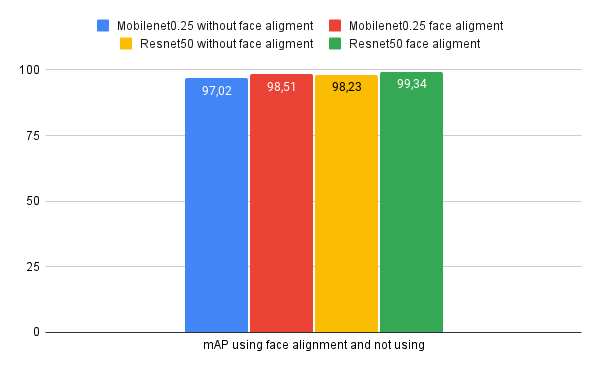
\includegraphics[width=0.4\textwidth]{gambar/facealigment.png}

  % Ubah sesuai dengan keterangan gambar yang diinginkan.
  \caption{mAP comparison between Mobilenet 0.25 and Resnet50 backbones using face alignment and not using face alignment}
  \label{fig:facealigment}
\end{figure}

From Figure \ref{fig:facealigment} in the face detection system based on the \emph{feature pyramid network}, Face alignment makes the accuracy increase by $1\%$. This increase occurred in the resnet50 and mobilenet0.25 backbones and occurred in all conditions, both day and night using 300W datasets \citep{sagonas2016300} \citep{sagonas2013300} \citep{sagonas2013semi}.

\begin{figure} [ht]
  \centering
  % Ubah sesuai dengan nama file gambar dan ukuran yang akan digunakan.
  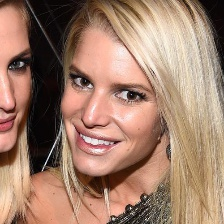
\includegraphics[width=0.2\textwidth]{gambar/beforefacealigment.jpg}
  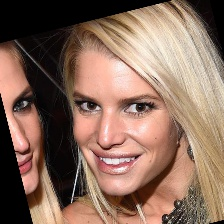
\includegraphics[width=0.2\textwidth]{gambar/afterfacealigment.jpg}

  % Ubah sesuai dengan keterangan gambar yang diinginkan.
  \caption{Comparison between before and after face alignment}
  \label{fig:beforeafterfacealigment}
\end{figure}

In Figure \ref{fig:beforeafterfacealigment}, An example of an image is shown before being processed using a face alignment and after being processed using a face alignment. It can be seen that the eyes that previously had different heights after the face alignment process became parallel to one another.

\subsection{Comparison with previous research}

In the previous research was detected using the same data but using a face detection system based on YOLO and SSD \citep{nugrohoevalution2016}.
It was also concluded from previous research that the SSD-based face detection system is able to provide
faster processing time and up to four times better FPS value than YOLO-based face detection systems. While the YOLO-based system
capable of delivering up to two times higher mAP values than SSD-based systems.

\begin{figure} [ht]
  \centering
  % Ubah sesuai dengan nama file gambar dan ukuran yang akan digunakan.
  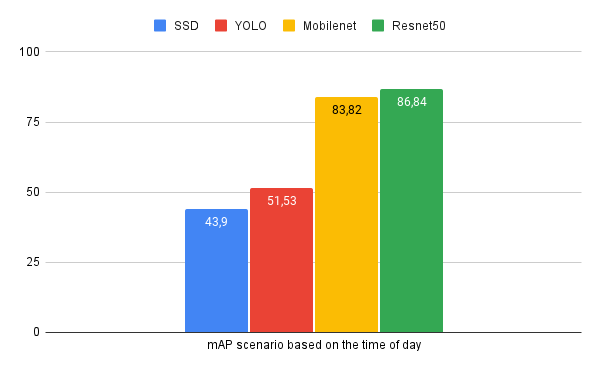
\includegraphics[width=0.4\textwidth]{gambar/perbandinganmapsiang.png}

  % Ubah sesuai dengan keterangan gambar yang diinginkan.
  \caption{Comparison of the mAP of the face detection system based on YOLO and SSD with the mAP of the face detection system based on backbone resnet50 and backbone mobilenet0.25 on noon time}
  \label{fig:perbandinganmapsiang}
\end{figure}

\begin{figure} [ht]
  \centering
  % Ubah sesuai dengan nama file gambar dan ukuran yang akan digunakan.
  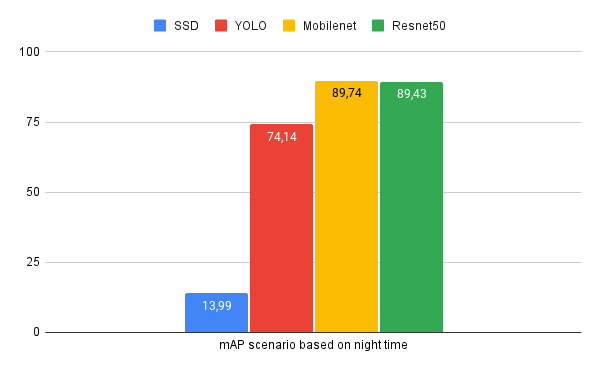
\includegraphics[width=0.4\textwidth]{gambar/perbandinganmapmalam.png}

  % Ubah sesuai dengan keterangan gambar yang diinginkan.
  \caption{Comparison of the mAP of the face detection system based on YOLO and SSD with the mAP of the face detection system based on backbone resnet50 and backbone mobilenet0.25 on night time}
  \label{fig:perbandinganmapmalam}
\end{figure}

From the comparison in Figure \ref{fig:perbandinganmapsiang} and Figures \ref{fig:perbandinganmapmalam}, it can be seen that the face detection system based on feature pyramid 
is superior to SSD and YOLO with 
the distance is quite far, Meanwhile backbone mobilenet0.25 is superior to backbone resnet50 with the mAP parameter if applied
in the feature pyramid-based face detection system.

\subsection{System Implementation Recommendations}

From all the test results that have been carried out, there are
several recommendations that can be applied so that the detection system 
feature pyramid-based faces can provide good detection performance, including:

\begin{itemize}
  \item Backbone mobilenet0.25 relatively usable in all conditions, With fast processing
  and accuracy that is not inferior to backbone resnet50, however backbone mobilenet0.25 has a weakness in that the search space is too narrow or too wide
  so it is recommended to use backbone mobilenet0.25 with a search space of 3-5 meters.
  \item The data that has been obtained shows that a good cctv placement condition is around 2.5-3 meters high with an elevation angle of $60^\circ$
  \item Detection at night the better the results if the environmental conditions where the detection is carried out
  provided additional lighting by using lamps.
  \item The best system recommendation, with reliable accuracy conditions using backbone resnet50 and a GPU with at least 4GB of VRAM.
\end{itemize}


  % Ubah judul dan label berikut sesuai dengan yang diinginkan.
\section{Kesimpulan}
\label{sec:kesimpulan}

% Ubah paragraf-paragraf pada bagian ini sesuai dengan yang diinginkan.

\lipsum[21-23]


  % Menampilkan daftar pustaka dengan format IEEE
  \bibliographystyle{IEEEtranN}
  \bibliography{pustaka/pustaka.bib}

  % Menyeimbangkan bagian akhir di kedua kolom
  \balance

\end{document}
